\documentclass{beamer}
\usepackage{tikz}
%\input{tikzall.tex} %包含所有的tikz包

\begin{document}
%
\begin{frame}
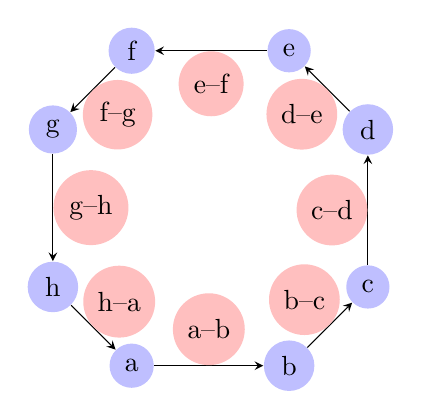
\begin{tikzpicture} [scale=1,auto=left,every node/.style={circle,fill=blue!25}]
	\node (a) at (-1,-2) {a};
	\node (b) at ( 1,-2) {b};
	\node (c) at ( 2,-1) {c};
	\node (d) at ( 2, 1) {d};
	\node (e) at ( 1, 2) {e};
	\node (f) at (-1, 2) {f};
	\node (g) at (-2, 1) {g};
	\node (h) at (-2,-1) {h};
	\foreach \from/\to in {a/b,b/c,c/d,d/e,e/f,f/g,g/h,h/a}
		\draw [-stealth] (\from) -- (\to) node[midway,fill=red!25] {\from--\to};
\end{tikzpicture}
\end{frame}

\end{document} 
